\documentclass{article}
\usepackage{graphicx} % Required for inserting images
\usepackage[preprint]{neurips_2024}
\usepackage{amsmath, amssymb, amsfonts}
\usepackage{hyperref}

\title{STAT 538 Final Project}
\author{Ghaleb Khalil, Andrew Wang}
\date{February 2026}

\usepackage[]{natbib}

\begin{document}

\maketitle

\section{Introduction}

Hidden Markov Models (HMMs) form one of the most important classes of probabilistic models for sequential data with underlying latent structure, with applications ranging from speech recognition to signal processing and financial time series prediction [1,2]. One of the key objectives of such applications is to study conformal prediction for structured sequential data inspired by Hidden Markov Models.

Conformal prediction provides a broad framework for prediction set construction with finite-sample, distribution-free guarantee of coverage [3,4,8]. While traditional conformal prediction techniques assume exchangeability of the underlying data, recent advances extend the framework to dependent data structures, including time series and latent variable models [6]. In particular, Nettasinghe et al. [7] proposed a conformal prediction framework for HMMs by exploiting the de Finetti representation of Markov chains, facilitating exact validity via admissible permutations of future observations. The key challenge with this approach, however, is that the resulting conformal prediction quantity involves averaging over all admissible permutations of future observations, whose number increases combinatorially with prediction horizon. In the HMM setting, each permutation involves computing likelihood-based quantities, typically requiring forward filtering, and thus becomes computationally intractable even for small prediction horizons.

In our paper, we propose a Monte Carlo approximation to the original conformal prediction quantity to overcome the computational intractability of the original approach. The key idea of our approach is to first express the original conformal prediction quantity as an expectation over a uniform distribution over all permutations and then replace the original approach of exhaustively enumerating all permutations with random sampling. While the original approach involves an exponentially large number of permutations to enumerate, our approach reduces the computational complexity to linear in the number of Monte Carlo samples.

We provide a theoretical justification of our approach by showing that our Monte Carlo approximation to the original conformal prediction quantity is unbiased and satisfies a non-asymptotic concentration inequality via Hoeffding’s inequality [5]. We further establish an approximate coverage guarantee by introducing an appropriate threshold adjustment, and characterize its asymptotic behavior, showing that the correction converges to the exact level at rate
\[
|t - \alpha| = O\left(\sqrt{\frac{\log M}{M}}\right).
\]

Finally, we present empirical results illustrating the computational advantages of the proposed method. In a sequential setting, we compare the evaluation of exhaustive permutation tests with Monte Carlo sampling under varying prediction horizons, showing significant reductions in execution times. The results verify that the combinatorial challenge of exact conformal prediction of hidden Markov models can indeed be replaced by an efficient approximation method without sacrificing theoretical validity, thus making the approach feasible in practice.
The implementation is available at:
\href{https://colab.research.google.com/drive/12J1AtzIR90r0Osa5-cmWRgQ2X8j_Xd24?usp=sharing}{Google Colab notebook}.

\section{Problem Formulation and Scope}

\subsection{Problem Formulation}

We formalize the conformal prediction framework for hidden Markov models following [7].

Let $x = (x_{t+1}, \ldots, x_{t+T})$ denote a candidate future discrete sequence obtained from clustering of length $T$, and let $\Pi$ denote the set of admissible permutations acting on future observations or blocks. For each permutation $\pi \in \Pi$, let $S(\pi)$ denote the associated conformity score, and let $I \in \Pi$ denote the identity permutation.

The conformal prediction procedure evaluates the quantity
\[
q(x) = \frac{1}{|\Pi|} \sum_{\pi \in \Pi} \mathbf{1}\{S(\pi) \ge S(I)\},
\]
which represents the proportion of permutations whose conformity score exceeds that of the identity. The conformal prediction set at level $1-\alpha$ is then defined as
\[
C_{1-\alpha} = \{x : q(x) > t\},
\]
where the threshold $t$ is chosen to ensure coverage at level $1-\alpha$.

A key limitation of this procedure is its computational cost. The evaluation of $q(x)$ requires enumeration over all permutations in $\Pi$, and the size of this set grows combinatorially with the prediction horizon $T$. As a result, exact conformal prediction becomes computationally infeasible even for moderate problem sizes.

\subsection{Scope of the Project}

The objective of this study is to address the computational bottleneck in the evaluation of $q(x)$ by replacing exhaustive permutation enumeration with a Monte Carlo approximation.

Specifically, the goals of this work are:
\begin{itemize}
\item Reformulate the conformal quantity $q(x)$ as an expectation under a uniform distribution over permutations;
\item Construct a Monte Carlo estimator based on i.i.d.\ samples from $\mathrm{Unif}(\Pi)$;
\item Establish theoretical properties of the estimator, including unbiasedness and concentration bounds;
\item Derive a threshold adjustment that preserves approximate coverage guarantees;
\item Characterize the asymptotic behavior of the estimation error;
\item Evaluate the computational efficiency of the proposed method empirically.
\end{itemize}

While we do not explicitly estimate parametric transition or emission distributions, the discrete structure obtained via clustering allows us to study the combinatorial aspects of conformal prediction in a controlled setting.
This formulation highlights the trade-off between computational efficiency and statistical guarantees, showing that the exponential complexity of exact conformal evaluation can be replaced by a controllable approximation with probabilistic guarantees.

\section{Monte Carlo Approximation for Conformal Prediction}

Let $\Pi$ denote the set of admissible permutations of the future blocks, and let $S(\pi)$ be the conformity score associated with permutation $\pi \in \Pi$. Let $I \in \Pi$ denote the identity permutation.

Define the exact conformal quantity:

\[
q(x) = \frac{1}{|\Pi|} \sum_{\pi \in \Pi} 1\{S(\pi) \ge S(I)\}.
\]

This quantity represents the proportion of permutations whose conformity score exceeds that of the identity, and is used to construct conformal prediction sets.

Further define the indicator variable:

\[
Z(\pi) = 1\{S(\pi) \ge S(I)\} \in \{0,1\}.
\]

Then the conformal quantity can be written as:

\[
q(x) = \frac{1}{|\Pi|} \sum_{\pi \in \Pi} Z(\pi).
\]

This representation allows us to interpret $q(x)$ as an expectation.

\textbf{Proposition 1 (Expectation Form).}
Let $\Pi^*$ be a random permutation drawn uniformly from $\Pi$,

\[
P(\Pi^* = \pi) = \frac{1}{|\Pi|}, \quad \forall \pi \in \Pi.
\]

Then:

\[
q(x) = E[Z(\Pi^*)].
\]

\textit{Proof.}
By definition of expectation over a finite discrete distribution,

\[
E[Z(\Pi^*)]
=
\sum_{\pi \in \Pi} Z(\pi)\, P(\Pi^* = \pi)
=
\frac{1}{|\Pi|} \sum_{\pi \in \Pi} Z(\pi)
=
q(x).
\quad
\]

\subsection{The Monte Carlo Estimator and its properties}

Motivated by the expectation representation, we define a Monte Carlo approximation of the score $\hat{q}$ calculated from sampling the permutation set.

Let $\Pi_1,\ldots,\Pi_M$ be i.i.d. samples from $\mathrm{Unif}(\Pi)$, and define:

\[
\hat{q}_M(x) = \frac{1}{M} \sum_{m=1}^M Z(\Pi_m).
\]

We identify and prove the unbiasedness of this estimator (\ref{unbiased}), the concentration bound (\ref{Concentration}), and then in the next section study the how the coverage of the resulting conformal set built on the Monte Carlo estimate of the score changes with respect to sample size.

\textbf{Proposition 2 (Unbiasedness).}\label{unbiased}

\[
E[\hat{q}_M(x)] = q(x).
\]

\textit{Proof.}
Using linearity of expectation,

\[
E[\hat{q}_M(x)]
=
\frac{1}{M} \sum_{m=1}^M E[Z(\Pi_m)].
\]

Since the $\Pi_m$ are i.i.d.,

\[
E[Z(\Pi_m)] = q(x),
\]

hence:

\[
E[\hat{q}_M(x)]
=
\frac{1}{M} \cdot M q(x)
=
q(x).
\quad
\]


The randomness in $\hat{q}_M(x)$ arises solely from the sampled permutations $\{\Pi_m\}_{m=1}^M$. Conditional on the observed data, the values $\{Z(\pi)\}_{\pi \in \Pi}$ are deterministic.

Thus, each

\[
X_m := Z(\Pi_m)
\]

is an i.i.d. Bernoulli random variable with mean $q(x)$, and satisfies:

\[
0 \le X_m \le 1.
\]

We therefore apply Hoeffding’s inequality.

\textbf{Theorem 1 (Concentration of the Monte Carlo Estimator).}\label{Concentration}
For any $\varepsilon > 0$,

\[
P\left(
\left|
\hat{q}_M(x) - q(x)
\right|
>
\varepsilon
\,\middle|\,
data
\right)
\le
2\exp(-2M\varepsilon^2).
\]

The randomness arises solely from permutation sampling; the conformity scores are deterministic given the data.

\textit{Proof.}
Since $X_1,\ldots,X_M$ are i.i.d., bounded in $[0,1]$, Hoeffding’s inequality yields:

\[
P\left(
\left|
\frac{1}{M}\sum_{m=1}^M X_m - E[X_m]
\right|
>
\varepsilon
\right)
\le
2\exp(-2M\varepsilon^2).
\]

Noting that $E[X_m] = q(x)$, the result follows. \hfill $\Box$

\subsection{Coverage under Monte Carlo Approximation}

The exact conformal prediction set is defined as:

\[
C_{1-\alpha} = \{x : q(x) > t\}.
\]

In practice, we use the Monte Carlo estimator:

\[
\hat{C}_{1-\alpha} = \{x : \hat{q}_M(x) > t\}.
\]

We now study how to choose $t$ so that coverage is preserved.

\textbf{Theorem 2 (Approximate Coverage Guarantee).} Let $\epsilon > 0$. If the threshold is chosen as
\[
t = \alpha - \epsilon,
\]
then:
\[
P\big(X_{\text{true}} \in \hat{C}_{1-\alpha}\big)
\ge 1 - \alpha - 2\exp(-2M\epsilon^2).
\]

\textit{Proof (Sketch).}
Let:

\[
A = \{q(X_{\mathrm{true}}) > \alpha \}, \quad
B = \{|\hat{q}_M(X_{\mathrm{true}}) - q(X_{\mathrm{true}})| \le \varepsilon\}.
\]

Then:

\[
P(A \cap B) \ge P(A) - P(B^c).
\]

From conformal validity, $P(A) \ge 1 - \alpha$, and from Theorem 1,

\[
P(B^c) \le 2\exp(-2M\varepsilon^2).
\]

On $A \cap B$, we have:

\[
\hat{q}_M(X_{\mathrm{true}})
\ge
q(X_{\mathrm{true}}) - \varepsilon
\ge
\alpha - \varepsilon.
\]

Choosing $t$ appropriately yields:

\[
\quad
P\big(X_{\text{true}} \in \hat{C}_{1-\alpha}\big)
\ge 1 - \alpha - 2\exp(-2M\epsilon^2).
\]

\subsection{Threshold Adjustment and Asymptotic Rate}

The concentration inequality implies that, to achieve accuracy $\varepsilon$ with probability at least $1 - \delta$, it suffices to choose:

\[
\epsilon = \sqrt{\frac{\log(2/\delta)}{2M}}
\]

Substituting into the threshold expression yields:

\[
|t - \alpha| = O\left(\sqrt{\frac{\log M}{M}}\right).
\]

Thus, as $M \to \infty$,

\[
t \to \alpha,
\quad \text{and} \quad
\hat{C}_{1-\alpha} \to C_{1-\alpha}.
\]

\section{Empirical Verification Methodology}

To evaluate the proposed Monte Carlo approximation, we compare it directly to the exact conformal prediction procedure under the same hidden-state prediction task used in \cite{nettasingheExtendingConformalPrediction2023}. We consider a discrete hidden-state setting with two latent states,
\[
\mathcal{X} = \{1,2\},
\]
which for real data can be obtained from a discretized representation of the observed sequence. For a future prediction horizon $T_1$, the candidate future hidden paths are given by
\[
\mathcal{C}_{T_1} = \mathcal{X}^{T_1},
\]
so that the number of candidate trajectories grows as
\[
|\mathcal{C}_{T_1}| = 2^{T_1}.
\]

The experiments are conducted for
\[
T_1 \in \{6,7,8,9,10\},
\]
which yields candidate path spaces ranging from 64 to 1024 possible future trajectories.

For each candidate path $x \in \mathcal{C}_{T_1}$, the exact conformal score $q(x)$ is first computed by exhaustively evaluating all admissible permutations of the future blocks. This exact computation serves as the benchmark and is performed once for each horizon, after which the resulting scores are stored and reused across all subsequent Monte Carlo comparisons.

The Monte Carlo approximation replaces exhaustive averaging over the admissible permutation set by random sampling. For each candidate path, we draw $M$ independent permutations uniformly from the admissible set and compute
\[
\hat q_M(x) = \frac{1}{M}\sum_{m=1}^M \mathbf{1}\{S(\Pi_m)\geq S(I)\},
\]
using the same conformity score as in the exact method. Thus, the only difference between the two procedures is the number of permutations evaluated.

Verification is performed pathwise by comparing $q(x)$ and $\hat q_M(x)$ over the full candidate path space. Estimation accuracy is summarized through mean absolute error and root mean squared error:
\[
\text{MAE} = \frac{1}{|\mathcal{C}_{T_1}|}\sum_{x\in\mathcal{C}_{T_1}} |\hat q_M(x)-q(x)|,
\]
\[
\text{RMSE} = \left(
\frac{1}{|\mathcal{C}_{T_1}|}\sum_{x\in\mathcal{C}_{T_1}} (\hat q_M(x)-q(x))^2
\right)^{1/2}.
\]

To evaluate whether approximation error affects the resulting prediction regions, exact and Monte Carlo conformal sets are constructed using the same threshold $t$:
\[
C^{\mathrm{exact}}_{1-\alpha} = \{x : q(x)>t\},
\qquad
\hat C^{\mathrm{MC}}_{1-\alpha} = \{x : \hat q_M(x)>t\}.
\]

Similarity between the two sets is measured using the Jaccard index,
\[
J(A,B)=\frac{|A\cap B|}{|A\cup B|},
\]
which provides a direct measure of how closely the approximate conformal set reproduces the exact prediction region.

Coverage is assessed by checking whether the true future hidden sequence belongs to each conformal set under both methods. This allows empirical comparison of whether the Monte Carlo approximation preserves the practical coverage behavior of the exact conformal procedure.

Finally, runtime is recorded separately for exact and Monte Carlo evaluation across all horizons. Because exact scores are reused once computed, the timing comparison isolates the marginal computational cost of exhaustive versus sampled permutation evaluation, allowing direct examination of how the two methods scale as the candidate path space increases.

\section{Results}

\subsection{Coverage}

We first check if the Monte Carlo approximation maintains the coverage level. We set $\alpha = 0.05$ and compute the empirical frequency that the true sequence falls within the Monte Carlo and exact conformal sets at different time horizons and with different sample sizes.

Empirical findings show that the Monte Carlo coverage closely tracks the exact coverage, with some deviations at smaller horizons due to finite-sample effects:

\begin{itemize}
\item $T1 = 6$: coverage = 0.65 (exact = MC)
\item $T1 = 7$: coverage = 0.95 (exact = MC)
\item $T1 = 8$: coverage = 0.90 (exact = MC)
\item $T1 = 9$: exact = 0.95, MC = 0.90
\item $T1 = 10$: coverage = 1.00 (exact = MC)
\end{itemize}

This shows that the Monte Carlo approximation maintains the coverage behavior of the exact approach, with small deviations at intermediate horizons. This observation is consistent with the theoretical approximate coverage guarantee provided in Section 3.

We then focus on the case of $T_1 = 9$. The empirical coverage of the Monte Carlo set is quite similar to the exact set, though perhaps more iterations are needed to demonstrate a clear pattern. It seems as if the true coverage of the Monte Carlo set is diminishing in the sample size, which is unexpected.

\begin{figure}[h]
\centering
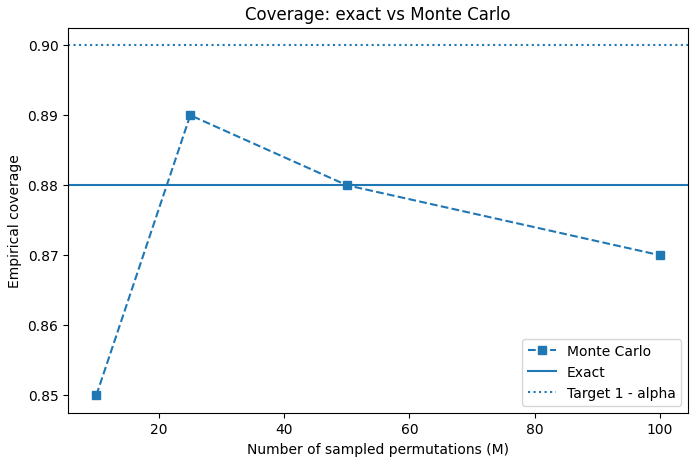
\includegraphics[width=0.6\textwidth]{Coverage.png}
\caption{Empirical coverage of the exact and Monte Carlo conformal methods $T_1 = 9$}
\end{figure}

\subsection{Convergence of the monte carlo estimator}

We now examine the accuracy of the Monte Carlo estimator $\hat{q}_M(x)$.

The mean absolute error and root-mean-square error (RMSE) between $\hat{q}_M(x)$ and $q(x)$ are small for all horizons: The mean absolute error increases monotonically from 0.0013 to 0.0125, while te RMSE increases from 0.0055 to 0.0248. This is as we expect: as the problem size increases with the horizon, the estimator variance increases slightly, though it remains well controlled. These results empirically validate the concentration result:
\[
\mid{\hat{q}}_M(x)-q(x)\mid=O\left(\sqrt{\frac{\log{M}}{M}}\right)
\]

\begin{figure}[h]
\centering
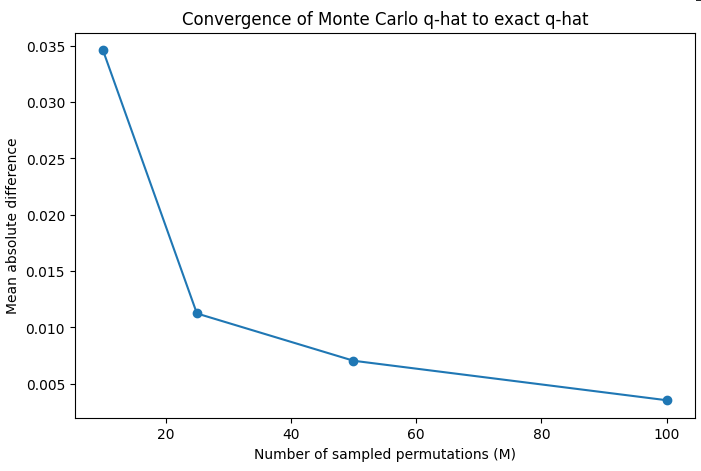
\includegraphics[width=0.6\textwidth]{Convergence.png}
\caption{Convergence of $\hat{q}_M(x)$ to $q(x)$. $T_1 = 9$}
\end{figure}

\subsection{Similarity of Conformal Sets}

To assess the effect of this approximation, we compute the similarity between exact and Monte Carlo conformal prediction sets using the Jaccard similarity measure. With a sample siz of 50 permutations, the range for the Jaccard similarity is between 0.990 and 1.000 at all time horizons. We can see that for the specific case of $T_1 = 9$, the convergence of the Monte Carlo set to the exact set is rapid. The results show that there is a very high similarity between exact and Monte Carlo conformal prediction sets.

\begin{figure}[h]
\centering
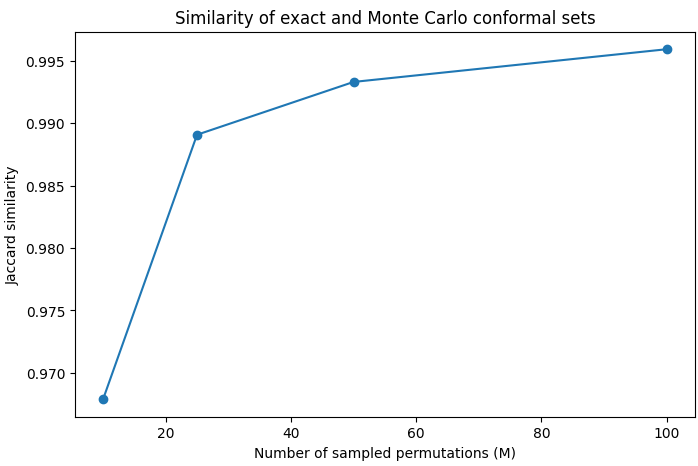
\includegraphics[width=0.6\textwidth]{Similarity.png}
\caption{Jaccard similarity between exact and Monte Carlo conformal sets. $T_1=9$}
\end{figure}

\subsection{Runtime and Computational Efficiency}

In the following, we analyze the efficiency of the methods. As one would expect, for small horizons $T1 = 6, 7, 8$, the Monte Carlo approach takes slightly longer. However, for larger horizons, the Monte Carlo approach becomes competitive, eventually faster. We were limited by computational power for the size of the horizons we could test, but the trend from these graphs indicates that the Monte Carlo approach should dominate the exact approach very quickly beyond $T_1=10$ (\ref{fig:runtimegrowth}).

Moreover, we also demonstrate that the Monte Carlo approach has linear runtime growth depending on the number of samples (\ref{fig:linearruntimeinM}).

\begin{figure}
    \centering
    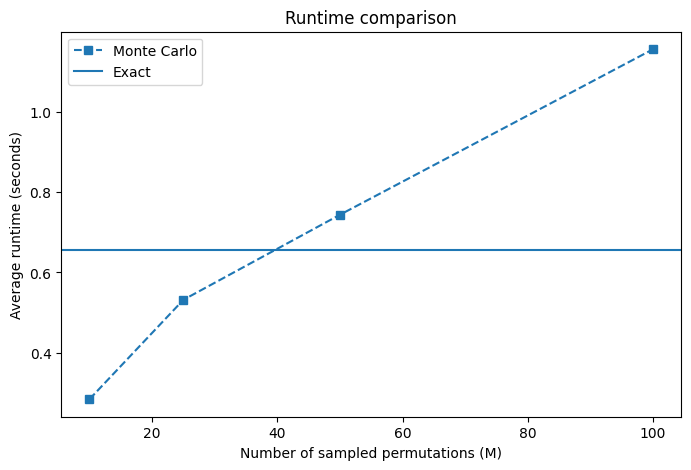
\includegraphics[width=0.5\linewidth]{Unknown.png}
    \caption{Linear runtime increase with sample size increase ($T_1=9$)}
    \label{fig:linearruntimeinM}
\end{figure}

\begin{figure}[h]
    \centering
    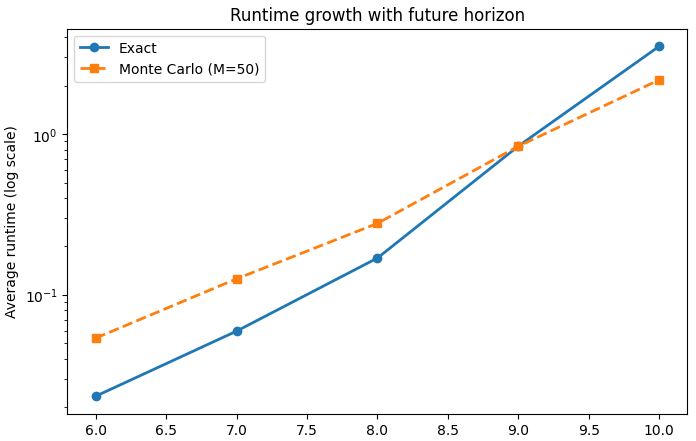
\includegraphics[width=0.6\textwidth]{Runtime growth scaled.png}
    \caption{Runtime comparison on a logarithmic scale.}
    \label{fig:runtimegrowth}
\end{figure}

\subsection{Discussion}

The Monte Carlo approximation replaces the exact computation of $q(x)$, which requires enumeration over $|\Pi|$ permutations, with an estimator based on $M$ samples.

Exact method complexity: $O(|\Pi| \cdot \text{cost per evaluation})$

Monte Carlo method: $O(M \cdot \text{cost per evaluation})$

Combined with the concentration result, this shows that exponential dependence on $|\Pi|$ can be replaced by a controllable approximation error that decays at rate:

\[
O\left(\sqrt{\frac{\log M}{M}}\right).
\]

This provides a practical and theoretically justified alternative to exhaustive conformal evaluation in high-dimensional or long-horizon settings.

by reducing the computational cost of conformal prediction on HMMs, our hope is that we can apply this algorithn to scenarios with a greater number of hidden states and to predict a higher number of periods (larger $T_1$). This enables broader application in predicting pricing and other financial indicators, which we plan to explore in a future extension of this project. moreover, this more efficient method for conformal prediction is useful beyond applications with large data sizes. In situations with relatively sparse data and moderate prediction length requirements, such as in the social sciences for predicting Macroeconomic or Political Economy indicators. In a future extension of this project, we plan to apply conformal prediction on HMMs using neural nets to the development of more powerful synthetic control experiments that are robust to treatment-induced changes in the structure of the data-generating process, something that is not well-accounted for in existing synthetic control methods.

\section{Appendix}
\appendix
\section{Detailed Proofs}

\subsection{Proof of Proposition 1}

Recall that

\[
Z(\pi)=1\{S(\pi)\ge S(I)\}, \qquad q(x)=\frac{1}{|\Pi|}\sum_{\pi\in\Pi} Z(\pi),
\]

and let $\Pi^* \sim \mathrm{Unif}(\Pi)$, so that

\[
P(\Pi^*=\pi)=\frac{1}{|\Pi|}, \qquad \forall \pi\in\Pi.
\]

We want to show that

\[
q(x)=E[Z(\Pi^*)].
\]

Since $\Pi^*$ is a discrete random variable supported on the finite set $\Pi$, its expectation is

\[
E[Z(\Pi^*)]
=
\sum_{\pi\in\Pi} Z(\pi)\,P(\Pi^*=\pi).
\]

Using the uniform distribution on $\Pi$,

\[
E[Z(\Pi^*)]
=
\sum_{\pi\in\Pi} Z(\pi)\frac{1}{|\Pi|}
=
\frac{1}{|\Pi|}\sum_{\pi\in\Pi} Z(\pi).
\]

By the definition of $q(x)$,

\[
\frac{1}{|\Pi|}\sum_{\pi\in\Pi} Z(\pi)=q(x).
\]

Therefore,

\[
E[Z(\Pi^*)]=q(x).
\]

This proves the result. \hfill $\Box$

\subsection{Proof of Proposition 2}

Recall that

\[
\hat{q}_M(x)=\frac{1}{M}\sum_{m=1}^M Z(\Pi_m),
\]

where

\[
\Pi_1,\ldots,\Pi_M \sim iid\,\mathrm{Unif}(\Pi).
\]

We want to prove that

\[
E[\hat{q}_M(x)]=q(x).
\]

Using linearity of expectation,

\[
E[\hat{q}_M(x)]
=
E\!\left[
\frac{1}{M}\sum_{m=1}^M Z(\Pi_m)
\right]
=
\frac{1}{M}\sum_{m=1}^M E[Z(\Pi_m)].
\]

Because all $\Pi_m$ are identically distributed as $\Pi^*\sim\mathrm{Unif}(\Pi)$, Proposition 1 gives

\[
E[Z(\Pi_m)]=q(x), \qquad m=1,\ldots,M.
\]

Substituting this into the previous display,

\[
E[\hat{q}_M(x)]
=
\frac{1}{M}\sum_{m=1}^M q(x)
=
\frac{1}{M}\cdot M q(x)
=
q(x).
\]

Hence $\hat{q}_M(x)$ is an unbiased estimator of $q(x)$. \hfill $\Box$

\subsection{Proof of Theorem 1}

Define

\[
X_m:=Z(\Pi_m), \qquad m=1,\ldots,M.
\]

Then

\[
\hat{q}_M(x)=\frac{1}{M}\sum_{m=1}^M X_m.
\]

We now explain carefully why Hoeffding’s inequality applies.

Conditional on the observed data, all conformity scores

\[
\{S(\pi):\pi\in\Pi\}
\]

are fixed deterministic real numbers. Therefore the indicator values

\[
Z(\pi)=1\{S(\pi)\ge S(I)\}, \qquad \pi\in\Pi,
\]

are also deterministic numbers in $\{0,1\}$.

Thus, conditional on the data, the only source of randomness is the sampling of the permutations

\[
\Pi_1,\ldots,\Pi_M.
\]

Since $\Pi_m\sim\mathrm{Unif}(\Pi)$, we have

\[
X_m=Z(\Pi_m)\in\{0,1\}.
\]

Hence

\[
0\le X_m\le 1.
\]

Also, because the $\Pi_m$ are i.i.d., the random variables $X_1,\ldots,X_M$ are i.i.d. conditional on the data.

Moreover,

\[
E[X_m\mid data]
=
E[Z(\Pi_m)\mid data]
=
\frac{1}{|\Pi|}\sum_{\pi\in\Pi} Z(\pi)
=
q(x),
\]

where the last equality follows from the definition of $q(x)$.

Thus, conditional on the data, $X_1,\ldots,X_M$ are i.i.d. bounded random variables with common mean $q(x)$.

Hoeffding’s inequality states that if $X_1,\ldots,X_M$ are independent and satisfy

\[
a_m\le X_m\le b_m,
\]

then for every $\varepsilon>0$,

\[
P\!\left(
\left|
\frac{1}{M}\sum_{m=1}^M X_m
-
\frac{1}{M}\sum_{m=1}^M E[X_m]
\right|
>
\varepsilon
\right)
\le
2\exp\!\left(
-\frac{2M^2\varepsilon^2}{\sum_{m=1}^M (b_m-a_m)^2}
\right).
\]

In our case, $a_m=0$ and $b_m=1$ for all $m$, so

\[
\sum_{m=1}^M (b_m-a_m)^2
=
\sum_{m=1}^M (1-0)^2
=
M.
\]

Therefore,

\[
P\!\left(
\left|
\frac{1}{M}\sum_{m=1}^M X_m
-
\frac{1}{M}\sum_{m=1}^M E[X_m]
\right|
>
\varepsilon
\,\middle|\,
data
\right)
\le
2\exp(-2M\varepsilon^2).
\]

Since

\[
\hat{q}_M(x)=\frac{1}{M}\sum_{m=1}^M X_m
\qquad \text{and} \qquad
E[X_m\mid data]=q(x),
\]

we obtain

\[
P\bigl(|\hat{q}_M(x)-q(x)|>\varepsilon \mid data\bigr)
\le
2\exp(-2M\varepsilon^2).
\]

This proves Theorem 1. \hfill $\Box$

\subsection{Detailed lower bound used for approximate coverage}

In the main text, the approximate conformal set is

\[
\hat{C}_{1-\alpha}=\{x:\hat{q}_M(x)>t\}.
\]

To study the probability that the true future sequence belongs to this set, let $X_{\mathrm{true}}$ denote the true future hidden sequence.

We begin with a general lower bound.

\textbf{Lemma A.1}

For any $t\in\mathbb{R}$ and any $\varepsilon>0$,

\[
P\bigl(X_{\mathrm{true}}\in \hat{C}_{1-\alpha}\mid data\bigr)
\ge
P\bigl(q(X_{\mathrm{true}})>t+\varepsilon \mid data\bigr)
-
2e^{-2M\varepsilon^2}.
\]

\textit{Proof}

Define the events

\[
A:=\{q(X_{\mathrm{true}})>t+\varepsilon\}, \qquad
B:=\{|\hat{q}_M(X_{\mathrm{true}})-q(X_{\mathrm{true}})|\le \varepsilon\}.
\]

We first show that

\[
A\cap B\subseteq \{X_{\mathrm{true}}\in \hat{C}_{1-\alpha}\}.
\]

Indeed, if $A\cap B$ occurs, then:

from $A$, we have $q(X_{\mathrm{true}})>t+\varepsilon$,

from $B$, we have $\hat{q}_M(X_{\mathrm{true}})\ge q(X_{\mathrm{true}})-\varepsilon$.

Combining the two inequalities,

\[
\hat{q}_M(X_{\mathrm{true}})
\ge
q(X_{\mathrm{true}})-\varepsilon
>
(t+\varepsilon)-\varepsilon
=
t.
\]

Hence

\[
\hat{q}_M(X_{\mathrm{true}})>t,
\]

which means

\[
X_{\mathrm{true}}\in \hat{C}_{1-\alpha}.
\]

Therefore,

\[
A\cap B\subseteq \{X_{\mathrm{true}}\in \hat{C}_{1-\alpha}\}.
\]

Taking probabilities gives

\[
P\bigl(X_{\mathrm{true}}\in \hat{C}_{1-\alpha}\mid data\bigr)
\ge
P(A\cap B\mid data).
\]

Now use the elementary inequality

\[
P(A\cap B)\ge P(A)-P(B^c).
\]

Thus,

\[
P\bigl(X_{\mathrm{true}}\in \hat{C}_{1-\alpha}\mid data\bigr)
\ge
P(A\mid data)-P(B^c\mid data).
\]

By definition of $B$,

\[
B^c=\{|\hat{q}_M(X_{\mathrm{true}})-q(X_{\mathrm{true}})|>\varepsilon\}.
\]

Applying Theorem 1 with $x=X_{\mathrm{true}}$ yields

\[
P(B^c\mid data)\le 2e^{-2M\varepsilon^2}.
\]

Therefore,

\[
P\bigl(X_{\mathrm{true}}\in \hat{C}_{1-\alpha}\mid data\bigr)
\ge
P\bigl(q(X_{\mathrm{true}})>t+\varepsilon \mid data\bigr)
-
2e^{-2M\varepsilon^2}.
\]

This proves the lemma. \hfill $\Box$

\subsection{Detailed proof of the approximate coverage statement}

To convert Lemma A.1 into a coverage guarantee, we need an explicit assumption on the exact conformal threshold.

\textbf{Assumption A.1 (Exact calibration condition)}

Suppose the exact conformal procedure is calibrated so that for some threshold level $\tau$,

\[
P\bigl(q(X_{\mathrm{true}})>\tau \mid data\bigr)\ge 1-\alpha.
\]

This assumption says that the exact conformal set

\[
C_{1-\alpha}^{exact}(\tau):=\{x:q(x)>\tau\}
\]

has conditional coverage at least $1-\alpha$.

\textbf{Theorem A.2}

Under Assumption A.1, if $t$ is chosen so that

\[
t+\varepsilon\le \tau,
\]

then

\[
P\bigl(X_{\mathrm{true}}\in \hat{C}_{1-\alpha}\mid data\bigr)
\ge
1-\alpha-2e^{-2M\varepsilon^2}.
\]

\textit{Proof}

From Lemma A.1,

\[
P\bigl(X_{\mathrm{true}}\in \hat{C}_{1-\alpha}\mid data\bigr)
\ge
P\bigl(q(X_{\mathrm{true}})>t+\varepsilon \mid data\bigr)
-
2e^{-2M\varepsilon^2}.
\]

If $t+\varepsilon\le \tau$, then

\[
\{q(X_{\mathrm{true}})>\tau\}\subseteq \{q(X_{\mathrm{true}})>t+\varepsilon\},
\]

because lowering the threshold only enlarges the event. Hence

\[
P\bigl(q(X_{\mathrm{true}})>t+\varepsilon \mid data\bigr)
\ge
P\bigl(q(X_{\mathrm{true}})>\tau \mid data\bigr).
\]

By Assumption A.1,

\[
P\bigl(q(X_{\mathrm{true}})>\tau \mid data\bigr)\ge 1-\alpha.
\]

Combining the inequalities,

\[
P\bigl(X_{\mathrm{true}}\in \hat{C}_{1-\alpha}\mid data\bigr)
\ge
1-\alpha-2e^{-2M\varepsilon^2}.
\]

This proves the theorem. \hfill $\Box$

\subsection{Detailed derivation of the threshold rate}

We now derive the asymptotic rate of the threshold error.

From Theorem A.2, the threshold $t$ is chosen so that
\[
t + \epsilon \le \tau,
\]
where $\tau$ is the exact conformal threshold satisfying
\[
P(q(X_{\text{true}}) > \tau \mid \text{data}) \ge 1 - \alpha.
\]

A natural choice is
\[
t = \tau - \epsilon,
\]

\[
|t - \tau| = \epsilon.
\]

From Theorem 1, to guarantee
\[
P\big(|\hat{q}_M(x) - q(x)| > \epsilon \mid \text{data}\big) \le \delta,
\]

\[
\epsilon = \sqrt{\frac{\log(2/\delta)}{2M}}.
\]

To obtain an explicit asymptotic rate, set
\[
\delta = M^{-1}.
\]

Then,
\[
\log(2/\delta) = \log(2M) = O(\log M),
\]

\[
\epsilon = \sqrt{\frac{\log(2M)}{2M}} = O\!\left(\sqrt{\frac{\log M}{M}}\right).
\]

Therefore,
\[
|t - \tau| = O\!\left(\sqrt{\frac{\log M}{M}}\right).
\]

If we identify $\tau = \alpha$, this yields
\[
|t - \alpha| = O\!\left(\sqrt{\frac{\log M}{M}}\right).
\]

This proves the rate. \hfill $\Box$

\subsection{Consequence for set convergence}

Because

\[
|t-\alpha|\to 0 \quad \text{as } M\to\infty,
\]

the Monte Carlo threshold converges to the exact threshold. Therefore, under regularity conditions that prevent instability at the boundary of the set, one expects the approximate conformal set

\[
\hat{C}_{1-\alpha}=\{x:\hat{q}_M(x)>t\}
\]

to approach the exact set

\[
C_{1-\alpha}=\{x:q(x)>\alpha\}.
\]

\section*{References}

\bibliography{ExportedItems}

{\small

\begin{enumerate}

\item L. R. Rabiner. 
A tutorial on hidden Markov models and selected applications in speech recognition. 
\textit{Proceedings of the IEEE}, 77(2):257--286, 1989.

\item O. Cappé, E. Moulines, and T. Rydén. 
\textit{Inference in Hidden Markov Models}. 
Springer, 2005.

\item V. Vovk, A. Gammerman, and G. Shafer. 
\textit{Algorithmic Learning in a Random World}. 
Springer, 2005.

\item G. Shafer and V. Vovk. 
A tutorial on conformal prediction. 
\textit{Journal of Machine Learning Research}, 9:371--421, 2008.

\item W. Hoeffding. 
Probability inequalities for sums of bounded random variables. 
\textit{Journal of the American Statistical Association}, 58(301):13--30, 1963.

\item V. Chernozhukov, K. Wüthrich, and Y. Zhu. 
Distribution-free predictive inference for time series. 
\textit{Journal of Econometrics}, 2021.

\item B. Nettasinghe, S. Chatterjee, R. Tripathy, and M. Halappanavar. 
Extending conformal prediction to hidden Markov models with exact validity via de Finetti’s theorem for Markov chains. 
\textit{Proceedings of the 40th International Conference on Machine Learning (ICML)}, 2023.

\item A. N. Angelopoulos and S. Bates. 
A gentle introduction to conformal prediction and distribution-free uncertainty quantification. 
\textit{Foundations and Trends in Machine Learning}, 2023.

\end{enumerate}

}

\end{document}
